\documentclass[12pt]{article}
\usepackage{amsmath}
\usepackage{amsfonts}
\usepackage{graphicx}
\usepackage[colorinlistoftodos]{todonotes}
\usepackage[utf8]{inputenc}
\usepackage{lmodern}
\usepackage[MeX]{polski}
\usepackage{rotating}
\usepackage{geometry}
\usepackage{multirow}
\usepackage{xcolor,colortbl}
\usepackage{xparse}
\usepackage[most]{tcolorbox}
\usepackage{fancyvrb,newverbs,xcolor}
\usepackage{amssymb}
\usepackage{booktabs}
\usepackage{float}
\usepackage{graphicx}
\graphicspath{{graphics/}}
\usepackage{minted}
\usepackage{tikz}
\usetikzlibrary{automata,arrows,positioning,calc}

\NewDocumentCommand{\newframedtheorem}{O{}momo}{%
\IfNoValueTF{#3}
{%
\IfNoValueTF{#5}
{\newtheorem{#2}{#4}}
{\newtheorem{#2}{#4}[#5]}%
}
{\newtheorem{#2}[#3]{#4}}
\tcolorboxenvironment{#2}{#1}%
}

\newframedtheorem{theorem}{Twierdzenie}[section]
\newframedtheorem{definition}[theorem]{Definicja}
\newframedtheorem{exercise}[theorem]{Zadanie}


\renewcommand{\figurename}{Załącznik}

\begin{document}

    \begin{titlepage}

        \newcommand{\HRule}{\rule{\linewidth}{0.5mm}}

        \center

        \textsc{\LARGE Uniwerystet Jagielloński}\\[1.5cm]

        \HRule \\[0.4cm]
        %        { \huge \bfseries ETL}\\[0.4cm]
        \textsc{\Large Pytania do egzaminu licencjackiego}\\[0.5cm]
        \textsc{\large na kierunku Informatyka}\\[0.5cm]
        \HRule \\[1.0cm]

        \Large% \emph{Autorzy:}\\
        Małgorzata \textsc{Dymek}\\[1.5cm]

        
\includegraphics[scale=0.27]{uj.jpg}\\[4cm]

        {\large Rok akademicki 2019/2020}\\

        \vfill
    \end{titlepage}

    \tableofcontents

    \newpage


    \begin{center}{\LARGE Matematyczne podstawy informatyki}\end{center}

    \section{Zasada indukcji matematycznej.}

    Przykład: $2^1 + 2^2 + \cdots + 2^n = 2^{n+1} - 2$, Nierówność Bernoulliego
    $dla ~ h \geq -1 ~~ (1+h)^2 \geq 1 + n*h, ~~ \forall n \in \mathbb{N}^{+}$, $1 + 2 + \cdots + n = \frac{n(n+1)}{2} \forall n \in \mathbb{N}$

    \newpage

    \section{Porządki częściowe i liniowe. Elementy największe, najmniejsze, maksymalne i minimalne.}

    Przykłady - sprawdź czy porządek: $xRy \Leftrightarrow x | y$

    \newpage

    \section{Relacja równoważności i zbiór ilorazowy.}

    Przykład: $xRy ~ \Leftrightarrow x \equiv_3 y$.

    \newpage

    \section{Metody dowodzenia twierdzeń: wprost, nie wprost, przez kontrapozycję.}

    \newpage

    \section{Metody numeryczne rozwiązywania równań nieliniowych: bisekcji, siecznych, Newtona.}

    \newpage

    \section{Rozwiązywanie układów równań liniowych: metoda eliminacji Gaussa, metody iteracyjne Jacobiego i Gaussa-Seidla.}

    \subsection{Metoda eliminacji Gaussa}

    Obliczając rząd macierzy metodą Gaussa należy za pomocą operacji elementarnych na wierszach sprowadzić macierz do
    macierzy schodkowej. Wtedy wszystkie niezerowe wiersze są liniowo niezależne i można łatwo odczytać rząd macierzy.

    \begin{align*}
        \begin{bmatrix}
            1 & -1 & 2 & 2\\
            2 & -2 & 1 & 0\\
            -1 & 2 & 1 & -2\\
            2 & -1 & 4 & 0
        \end{bmatrix}
        \stackrel{w_2 - 2w_1, w_3 + w_1, w_4 - 2w_1}{\sim}
        \begin{bmatrix}
            1 & -1 & 2 & 2\\
            0 & 0 & -3 & -4\\
            0 & 1 & 3 & 0\\
            0 & 1 & 0 & -4
        \end{bmatrix}
        \stackrel{w_2 \leftrightarrow w_3}{\sim}
        \begin{bmatrix}
            1 & -1 & 2 & 2\\
            0 & 1 & 3 & 0\\
            0 & 0 & -3 & -4\\
            0 & 1 & 0 & -4
        \end{bmatrix}
        \sim
    \end{align*}

    \begin{align*}
        \stackrel{w4 - w_2}{\sim}
        \begin{bmatrix}
            1 & -1 & 2 & 2\\
            0 & 1 & 3 & 0\\
            0 & 0 & -3 & -4\\
            0 & 0 & -3 & -4
        \end{bmatrix}
        \stackrel{w4 - w_3}{\sim}
        \begin{bmatrix}
            1 & -1 & 2 & 2\\
            0 & 1 & 3 & 0\\
            0 & 0 & -3 & -4\\
            0 & 0 & 0 & 0
        \end{bmatrix}
    \end{align*}

    \hfill \\
    \begin{center}{\large Metody iteracyjne}\end{center}
    Ogólna postać metody iteracyjnej:
    \begin{align*}
        Ax = b
    \end{align*}
    \begin{align*}
        Qx^{n+1} = (Q - A)x^n + b = \tilde{b}
    \end{align*}

    \begin{align*}
        x^0 = (0,0,0)
    \end{align*}
    \begin{align*}
        \begin{bmatrix}
            5 & -2 & 3\\
            2 & 4 & 2\\
            2 & -1 & -4\\
        \end{bmatrix}
        \begin{bmatrix}
            x_1\\
            x_2\\
            x_3\\
        \end{bmatrix}
        =
        \begin{bmatrix}
            10\\
            0\\
            0\\
        \end{bmatrix}
    \end{align*}
    \begin{align*}
        \left\{\begin{matrix}
                   5x_1 + (-2)x_2 + 3x_3 = 10\\
                   2x_1 + 4x_2 + 2x_3 = 0\\
                   2x_1 + (-1)x_2 + (-4)x_3 = 0\\
        \end{matrix}\right.
    \end{align*}

    \subsection{Metoda iteracyjna Jacobiego}

    \subsubsection{Algebraicznie}
    \begin{align*}
        \left\{\begin{matrix}
                   x^{N+1}_1 = \frac{1}{5}(10 + 2x^N_2 - 3x^N_3)\\
                   x^{N+1}_2 = \frac{1}{4}(-2x^N_1 - 2x^N_3)\\
                   x^{N+1}_3 = -\frac{1}{4}(x^N_2 - 2x^N_1)
        \end{matrix}\right.
    \end{align*}

    \subsubsection{Macierzowo}
    \begin{align*}
        Q = D ~~ \text{(diagonalna)}
    \end{align*}

    \subsection{Metoda iteracyjna Gaussa-Seidla}
    \subsubsection{Algebraicznie}
    \begin{align*}
        \left\{\begin{matrix}
                   x^{N+1}_1 = \frac{1}{5}(10 + 2x^N_2 - 3x^N_3)\\
                   x^{N+1}_2 = \frac{1}{4}(-2x^N_1 - 2x^{N+1}_3)\\
                   x^{N+1}_3 = -\frac{1}{4}(x^{N+1}_2 - 2x^{N+1}_1)
        \end{matrix}\right.
    \end{align*}

    \subsubsection{Macierzowo}
    \begin{align*}
        Q = L + D ~~ \text{(diagonalna i dolnotrójkątna)}
    \end{align*}


    \newpage

    \section{Wartości i wektory własne macierzy: numeryczne algorytmy ich wyznaczania.}

    \newpage

    \section{Interpolacja wielomianowa: metody Lagrange'a i Hermite'a. Efekt Rungego.}

    \newpage

    \section{Zmienne losowe dyskretne. Definicje i najważniejsze rozkłady.}

    \newpage

    \section{Zmienne losowe ciągłe. Definicje i najważniejsze rozkłady.}

    \subsection{Rozkład jednostajny}
    \begin{exercise}
        Zmienna losowa X ma rozkład jednostajny na odcinku [2, 6]. Wykonaj
        polecenia:
        \begin{enumerate}
            \item zapisz wzór na gęstość zmiennej losowej X
            \item oblicz prawdopodobieństwo zdarzenia że $X\in[3,3.5]$
            \item oblicz prawdopodobieństwo zdarzenia że $X \in (3,3.5)$
        \end{enumerate}
    \end{exercise}
    Rozwiązanie:

    \begin{enumerate}
        \item wzór na gęstość zmiennej losowej X to
        \begin{align*}
            \chi_{[2,6]}(x) = \left\{\begin{matrix}
                                         \frac{1}{4} ~~ \text{gdy} ~ x \in [2,6]  \\
                                         0 ~~ \text{gdy} ~ x \notin [2,6]  \\
            \end{matrix}\right.
        \end{align*}
        \item prawdopodobieństwo zdarzenia, że $X \in [3, 3.5]$ to
        \begin{align*}
            P(X \in [3, 3.5]) = \int_3^{3.5} \frac{1}{4} dx = \frac{1}{4} (3.5 - 4) = \frac{1}{8}
        \end{align*}
        \item prawdopodobieństwo zdarzenia że $X \in {3, 3.5}$ to
        \begin{align*}
            P(X \in (3, 3.5)) = P(X \in [3, 3.5]) = \frac{1}{8}
        \end{align*}
    \end{enumerate}

    \subsection{Rozkład wykładniczy}
    \begin{exercise}
        Zmienna losowa X ma rozkład wykładniczy z parametrem $\lambda = 1$. Wykonaj
        polecenia:
        \begin{enumerate}
            \item narysuj gęstość/ zapisz wzór na gęstość zmiennej losowej X
            \item na powyższym rysunku przedstaw prawdopodobieństwo zdarzenia że $X\in[0,1]$
            \item oblicz prawdopodobieństwo zdarzenia że $X \in [0,1]$
        \end{enumerate}
    \end{exercise}
    Rozwiązanie:\\


    \textbf{Punkty 1 i 2}:
    \begin{figure}[H]
        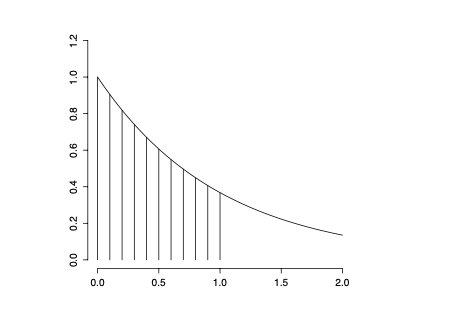
\includegraphics[width=\linewidth]{10_2.png}
    \end{figure}

    \textbf{Punkt 3} - prawdopodobieństwo zdarzenia że $X \in [0,1]$ wynosi
    \begin{align*}
        P(X \in [0,1]) = \int_0^1 f(x) dx = \int_0^1 e^{-x} dx = [-e^{-x}]_{x=0}^{x=1} = 1 - e^{-1}
    \end{align*}


    \subsection{Rozkład normalny}
    \begin{exercise}
        Zmienna losowa X ma rozkład normalny o parametrach $\mu = 0$ oraz $\sigma = 1$. Podaj prawdopodobieństwo, że
        X osiąga wartości dodatnie.
    \end{exercise}
    Rozwiązanie:\\

    Wykres tej funkcji jest parzysty, a pole calego wykresu wynosi 1 więc z połowy jest $\frac{1}{2}$.
    \begin{align*}
        P(X > 0) =  \int_o^{\infty} f(x)dx = \frac{1}{2}
    \end{align*}

    \subsection{Rozkład Gamma, Wzór Gamma-Poisona}
    \begin{exercise}
        Kompilacja programu składa się z 3 części przetwarzanych przez kompilator sekwencyjnie,jedna po drugiej.
        Czas przetwarzania każdej z części ma rozkład wykładniczy ze średnim czasem 5 minut, niezależnym od
        czasu przetwarzania pozostałych części.
        \begin{enumerate}
            \item oblicz wartość oczekiwaną i wariancję całkowitego czasu kompilacji
            \item oblicz prawdopodobieństwo, że cały proces kompilacji zostanie przeprowadzony w
            czasie mniejszym niż 12 minut.
        \end{enumerate}
    \end{exercise}
    Rozwiązanie:\\

    Całkowity czas kompilacji opisuje zmienna losowa o rozkładzie $Gamma(T \sim \Gamma(\alpha = 3, \lambda = \frac{1}{5}))$.
    Wartość oczekiwana i wariancja całkowitego czasu kompilacji to
    \begin{align*}
        E(X) = \frac{\alpha}{\lambda} = \frac{3}{\frac{1}{5}} = 15
    \end{align*}
    \begin{align*}
        Var(x) = \frac{\alpha}{\lambda^2} = \frac{3}{\frac{1}{25}}= 75
    \end{align*}

    Prawdopodobieństwo, że cały proces kompilacji zostanie przeprowadzony w
    czasie mniejszym niż 12 minut liczymy korzystając z formuły Gamma-Poisona.
    \begin{align*}
        P(T < t) = P(X \geq \alpha),
    \end{align*}
    gdzie $X \sim Poisson(\lambda*t = \frac{1}{5} * 12 = 2.4)$ oraz $\alpha = 3$, $t = 12$. Mamy więc:
    \begin{align*}
        P(T < 12) = P (X \geq 3) = 1 - P(0) - P(1) - P(2) = 1 - F_X(2) = 1 - 0.5697 = 0.43
    \end{align*}

    \newpage

    \section{Łancuchy Markowa. Rozkład stacjonarny.}
    \begin{exercise}
        W pewnym mieście każdy dzień jest słoneczny albo deszczowy. Po dniu słonecznym dzień słoneczny
        następuje z prawdopodobieństwem 0.7, a po dniu deszczowym z prawdopodobieństwem 0.4.
        \begin{enumerate}
            \item Narysuj łańcuch markowa oraz wyznacz macierz przejścia dla niego.
            \item W poniedziałek padało. Stwórz prognozę na wtorek, środę i czwartek.
            \item Meteorolodzy przewidują 80\% szans na deszcz w poniedziałek. Stwórz prognozę na wtorek, środę i czwartek.
            \item Znajdź rozkład stacjonarny.
        \end{enumerate}
    \end{exercise}

    \begin{enumerate}
        \item Łańcuch Markowa:
        \begin{center}
            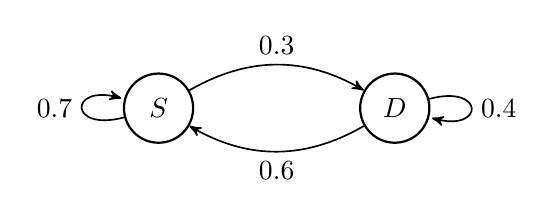
\begin{tikzpicture}[->, >=stealth', auto, semithick, node distance=3cm]
                \tikzstyle{every state}=[fill=white,draw=black,thick,text=black,scale=1]
                \node[state]    (S)                     {$S$};
                \node[state]    (D)[right of=S]   {$D$};
                \path
                (S) edge[loop left]     node{$0.7$}         (S)
                edge[bend left,above]      node{$0.3$}      (D)
                (D) edge[loop right]    node{$0.4$}     (D)
                edge[bend left,below]     node{$0.6$}         (S);
            \end{tikzpicture}

            Macierz przejść:
            \begin{align*}
                \begin{bmatrix}
                    0.7 & 0.3\\
                    0.4 & 0.6
                \end{bmatrix}
            \end{align*}
        \end{center}
        \item \hfill \\
        Wtorek:
        \begin{align*}
            \begin{bmatrix}
                0 & 1
            \end{bmatrix}
            \begin{bmatrix}
                0.7 & 0.3\\
                0.4 & 0.6
            \end{bmatrix}
            =
            \begin{bmatrix}
                0.4 & 0.6
            \end{bmatrix}
        \end{align*}
        Środa:
        \begin{align*}
            \begin{bmatrix}
                0.4 & 0.6
            \end{bmatrix}
            \begin{bmatrix}
                0.7 & 0.3\\
                0.4 & 0.6
            \end{bmatrix}
            =
            \begin{bmatrix}
                0.52 & 0.48
            \end{bmatrix}
        \end{align*}
        Czwartek:
        \begin{align*}
            \begin{bmatrix}
                0.52 & 0.48
            \end{bmatrix}
            \begin{bmatrix}
                0.7 & 0.3\\
                0.4 & 0.6
            \end{bmatrix}
            =
            \begin{bmatrix}
                0.556 & 0.444
            \end{bmatrix}
        \end{align*}
        \item \hfill \\
        Wtorek:
        \begin{align*}
            \begin{bmatrix}
                0.2 & 0.8
            \end{bmatrix}
            \begin{bmatrix}
                0.7 & 0.3\\
                0.4 & 0.6
            \end{bmatrix}
            =
            \begin{bmatrix}
                0.46 & 0.54
            \end{bmatrix}
        \end{align*}
        Środa:
        \begin{align*}
            \begin{bmatrix}
                0.46 & 0.54
            \end{bmatrix}
            \begin{bmatrix}
                0.7 & 0.3\\
                0.4 & 0.6
            \end{bmatrix}
            =
            \begin{bmatrix}
                0.538 & 0.462
            \end{bmatrix}
        \end{align*}
        Czwartek:
        \begin{align*}
            \begin{bmatrix}
                0.538 & 0.462
            \end{bmatrix}
            \begin{bmatrix}
                0.7 & 0.3\\
                0.4 & 0.6
            \end{bmatrix}
            =
            \begin{bmatrix}
                0.5614 & 0.4386
            \end{bmatrix}
        \end{align*}
        \item Macierz przejść:
        \begin{align*}
            \begin{bmatrix}
                0.7 & 0.3\\
                0.4 & 0.6
            \end{bmatrix}
        \end{align*}
        Rozwiązujemy układ równań:
        \begin{align*}
            \left\{\begin{matrix}
                       \pi P = \pi\\
                       \pi_1 + \pi_2 = 1
            \end{matrix}\right.
        \end{align*}
        \begin{align*}
            \pi P =
            \begin{bmatrix}
                \pi_1 & \pi_2
            \end{bmatrix}
            \begin{bmatrix}
                0.7 & 0.3\\
                0.4 & 0.6
            \end{bmatrix}
            =
            \begin{bmatrix}
                0.7\pi_1 + 0.4\pi_2 & 0.3\pi_1 + 0.6\pi_2
            \end{bmatrix}
        \end{align*}
        \begin{align*}
            \left\{\begin{matrix}
                       0.7\pi_1 + 0.4\pi_2 = \pi_1\\
                       0.3\pi_1 + 0.6\pi_2 = \pi_2\\
                       \pi_1 + \pi_2 = 1
            \end{matrix}\right.
        \end{align*}
        Stąd otrzymujemy
        \begin{align*}
            \begin{bmatrix}
                \pi_1 & \pi_2
            \end{bmatrix}
            =
            \begin{bmatrix}
                \frac{4}{7} & \frac{3}{7}
            \end{bmatrix}
        \end{align*}
    \end{enumerate}
    \newpage

    \section{Testy statystyczne: test z, test t-Studenta, test chi-kwadrat.}
    Generalnie:
    \begin{itemize}
        \item Z-testów używamy do sprawdzenia czy testowana próba pasuje do zadanej populacji lub do porównywania dwóch \textbf{dużych} (n > 30) prób
        \item T-testów używamy do porównywania dwóch \textbf{małych} (n < 30) prób testowych ze sobą
        \begin{itemize}
            \item Próby mogą być niezależne - np. wyniki sprawdzianów w dwóch grupach
            \item Mogą być również zależne (dotyczyć jednej i tej samej grupy) - np. waga przed zastosowaniem diety i po
            \item Może również służyć do porównywania próby do zadanej wartości (np. średniej) - podobnie jak Z-testy (?)
        \end{itemize}
        \item Chi-kwadrat używamy do ustalania \texttt{goodness of fit} dla próbki względem populacji lub do zbadania niezależności
    \end{itemize}

    \subsection{Z-test}
    \begin{exercise}
        Inżynier jakości znajduje 10 wadliwych produktów w próbie 500 egzemplarzy pewnego komponentu od wytwórcy A. Wśród 400 egzemplarzy od wytwórcy B znajduje 12 wadliwych. Firma komputerowa, korzystająca z tych komponentów twierdzi, że jakość wyrobów od obu producentów jest taka sama. Sprawdź, czy na 5\% poziomie istotności istnieją wystarczające dowody do odrzucenia tego twierdzenia.
    \end{exercise}

    $H_{0}$: Jakość wyrobów obu producentów jest taka sama \\

    $H_{a}$: Jakość wyrobów obu producentów jest różna \\

    Obliczamy proporcje dla obu prób:
    \begin{equation*}
        p_{1} = \frac{10}{500} = \frac{1}{50}
    \end{equation*}
    \begin{equation*}
        p_{2} = \frac{12}{400} = \frac{3}{100}
    \end{equation*}

    oraz proporcję dla \texttt{próby połączonej}:
    \begin{equation*}
        \bar{p} = \frac{10 + 12}{500 + 400} = \frac{11}{450}
    \end{equation*}

    Następnie używamy wzoru:
    \begin{equation*}
        Z = \frac{p_{1} - p_{2}}{\sqrt{\bar{p}(1-\bar{p})(\frac{1}{n_{1}} + \frac{1}{n_{2}})}}
    \end{equation*}
    \begin{equation*}
        Z = \frac{\frac{1}{50} - \frac{3}{100}}{\sqrt{\frac{11}{450}(1-\frac{11}{450})(\frac{1}{500} + \frac{1}{400})}} = \frac{-\frac{1}{100}}{\sqrt{\frac{4829}{45000000}}} \approx -0.9653
    \end{equation*} \\

    Odczytujemy z tablic dla Z-testów wartość dla \texttt{-0.9653} i jest to \textbf{0.1685} \\

    W naszej hipotezie mamy pytanie o równość więc bierzemy pod uwagę obie końcówki przedziału (?). Mamy sprawdzić prawdziwość naszej hipotezy na 5\% poziomie istotności, więc na każdą końcówkę mamy po 2.5\%. \\

    0.1685 $<$ 2.5 więc możemy odrzucić hipotezę zerową twierdząc, że jakość wyrobów obu producentów jest różna


    \subsection{T-testy}
    \begin{exercise}
        Posiadacz konta internetowego, w długim okresie czasu, w trakcie logowania pisze swój login i hasło z przerwami pomiędzy kolejnymi wciśnięciami klawiszy wynoszącymi 0.2s. Pewnego dnia zarejestrowane logowanie na to konto z prawidłowym hasłem, przy czym czasy odstępów pomiędzy wciśnięciami kolejnych klawiszy wynosiły: \\

        .24, .22, .26, .34, .35, .32, .33, .29, .19, .36, .30, .15, .17, .20, .28, .40, .37, .27 sekund \\

        Na 5\% poziomie ufności zweryfikuj, czy dane te mogą być dowodem na nieautoryzowany dostęp do konta?
    \end{exercise} 

    $H_{0}$: Dostęp do konta jest autoryzowany \\

    $H_{a}$: Dostęp do konta jest nieautoryzowany \\

    Korzystamy ze wzoru:
    \begin{equation*}
        T = \frac{\bar{x} - \mu_{0}}{\sigma}\sqrt{n}
    \end{equation*}

    gdzie:
    \begin{itemize}
        \item $\bar{x}$ - średnia z badanej próby
        \item $\mu_{0}$ - zakładana średnia
        \item $\sigma$ - odchylenie standardowe z próby
        \item n - wielkość próby
    \end{itemize}

    W naszym przypadku:

    \begin{gather}
        \bar{x} \approx 0.28 \\
        \mu_{0} = 0.2 \\
        \sigma \approx 0.07324 \\
        n = 18
    \end{gather}

    Podstawiając do wzoru mamy:
    \begin{equation*}
        T = \frac{0.28 - 0.2}{0.07324}\sqrt{18} \approx 4.63423341
    \end{equation*}

    Ilość naszych stopni swobody to n-1 więc w naszym przypadku 17 \\

    Odczytujemy z tablic rozkładu t-studenta wartość odpowiadającą 2.5\% poziomowi ufności (5\%/2) oraz 17 stopniom swobody i jest to \textbf{2.11} \\

    Ponieważ 4.63423341 $>$ 2.11 nie mamy podstawy aby odrzucić hipotezę zerową


    \subsection{Testy Chi-kwadrat}
    \begin{exercise}
        Producent kostki do gry deklaruje, że oczka na jego \texttt{niesprawiedliwej} kostce wypadają z następującym prawdopodobieństwem:
        \begin{itemize}
            \item 1 oczko - $\frac{1}{2}$
            \item 2 oczka - $\frac{1}{4}$
            \item 3 oczka - $\frac{1}{25}$
            \item 4 oczka - $\frac{1}{50}$
            \item 5 oczek - $\frac{1}{25}$
            \item 6 oczek - $\frac{3}{20}$
        \end{itemize}
        Dla 100 rzutów zaobserwowano natomiast nastepujące wyniki:
        \begin{itemize}
            \item 1 oczko - 55 razy
            \item 2 oczka - 20 razy
            \item 3 oczka - 6 razy
            \item 4 oczka - 3 razy
            \item 5 oczek - 2 razy
            \item 6 oczek - 14 razy
        \end{itemize}
        Przeprowadź test zgodności (\texttt{goodness of fit}) $\chi^{2}$ i  rozstrzygnij na poziomie 5\% istotności czy producent ma rację
    \end{exercise}

    Wyliczamy wartości oczekiwane dla każdego przedziału i zgodnie z \texttt{rule of thumb} w razie potrzeby je łączymy tak, aby dla każdego z nich wartość była $\geq$ 5

    \begin{table}[H]
        \centering
        \begin{tabular}{|c|c|c|c|c|c|}
        \hline
        n & $Obs_{n}$ & $Exp_{n}$ & x                  & $Obs_{x}$           & $Exp_{x}$           \\ \hline
        1 & 55        & 50        & 1                  & 55                  & 50                  \\ \hline
        2 & 20        & 25        & 2                  & 20                  & 25                  \\ \hline
        3 & 6         & 4         & \multirow{3}{*}{3} & \multirow{3}{*}{11} & \multirow{3}{*}{10} \\ \cline{1-3}
        4 & 3         & 2         &                    &                     &                     \\ \cline{1-3}
        5 & 2         & 4         &                    &                     &                     \\ \hline
        6 & 14        & 15        & 4                  & 14                  & 15                  \\ \hline
        \end{tabular}
    \end{table}

    Następnie aby obliczyć $\chi^{2}$ stosujemy następujący wzór (N to liczba naszych x):
    \begin{equation*}
        \chi^{2} = \sum_{x=1}^{N} \frac{(Obs_{x} - Exp_{x})^{2}}{Exp_{x}}
    \end{equation*}

    W naszym przypadku $\chi^{2} \approx 1.6666$ \\

    Stopnie swobody obliczamy ze wzoru \textbf{N -1}, gdzie N to liczba naszych x-ów. W naszym przypadku liczba stopni swobody jest więc równa \textbf{3}. \\

    Następnie odczytujemy z tablicy $\chi^{2}$ wartość dla 5\% istotności przy 3 stopniach swobody. Jest ona równa \textbf{7.82} \\

    1.6666 $<$ 7.82 stąd nie mamy więc podstawy do odrzucenia hipotezy zerowej

    \newpage






    \section{Wzór Bayesa i jego interpretacja.}
    \begin{exercise}
        W firmie IT 20\% wytwarzanych modułów przechodzi specjalny proces inspekcji. Z danych historycznych wiadomo, że każdy moduł poddany inspekcji nie ma defektów z prawdopodobieństwem 0.95. Dla modułu nie poddanego procesowi inspekcji prawdopodobieństwo to wynosi jedynie 0.7. Klient znalazł defekt w module. Jakie jest prawdopodobieństwo, że moduł ten przeszedł przez proces inspekcji?
    \end{exercise}

    Korzystamy oczywiście ze wzoru Bayesa:
    \begin{equation*}
        P(A|B) = \frac{P(B|A)P(A)}{P(B)} ~ ~ ~ ~ \text{przy $P(B) > 0$}
    \end{equation*} \\

    I - moduł przeszedł przez inspekcję \\
    D - moduł ma defekt \\

    $P(I) = \frac{20}{100} = \frac{1}{5} ~ ~ ~ ~ P(\bar{I}) = \frac{4}{5}$ \\

    $P(\bar{D}|I) = \frac{95}{100} = \frac{19}{20} ~ ~ ~ ~ P(D|I) = \frac{1}{20}$ \\

    $P(\bar{D}|\bar{I}) = \frac{70}{100} = \frac{7}{10} ~ ~ ~ ~ P(D|\bar{I}) = \frac{3}{10}$ \\

    \begin{equation*}
        P(I|D) = \frac{P(D|I)\cdot P(I)}{P(D)} = \frac{P(D|I)\cdot P(I)}{P(D|I)\cdot P(I) + P(D|\bar{I})\cdot P(\bar{I})} = \frac{\frac{1}{20}\cdot \frac{1}{5}}{\frac{1}{20}\cdot \frac{1}{5} + \frac{3}{10}\cdot \frac{4}{5}} = \frac{1}{25}
    \end{equation*}

    Prawdopodobieństwo że moduł, w którym znalazł się defekt przeszedł proces inspekcji wynosi $\frac{1}{25}$.

    \newpage





    \section{Istnienie elementów odwrotnych względem mnożenia w strukturze $(Zm, +, *)$ w zależności od liczby naturalnej m. Rozszerzony algorytm Euklidesa.}
    \section{Ortogonalność wektorów w przestrzeni $R_n$; związki z liniową niezależnością. Metoda ortonormalizacji Grama-Schmidta.}

    \newpage

    \section{Liczby Stirlinga I i II rodzaju i ich interpretacja.}

    \newpage

    \section{Twierdzenia Eulera i Fermata; funkcja Eulera.}

    \newpage

    \section{Konfiguracje i t-konfiguracje kombinatoryczne.}

    \newpage

    \section{Cykl Hamiltona, obwód Eulera, liczba chromatyczna - definicje i twierdzenia.}

    \newpage

    \section{Algorytm Forda-Fulkersona wyznaczania maksymalnego przepływu.}
    \section{Rozwiązywanie równan rekurencyjnych przy użyciu funkcji tworzących (generujących) oraz przy użyciu równania charakterystycznego.}

    \newpage

    \section{Ciąg i granica ciągu liczbowego, granica funkcji.}

    \newpage

    \section{Ciągłość i pochodna funkcji. Definicja i podstawowe twierdzenia.}

    \newpage

    \section{Ekstrema funkcji jednej zmiennej. Definicje i twierdzenia.}

    \newpage

    \section{Całka Riemanna funkcji jednej zmiennej.}

    \newpage

    \section{Pochodne cząstkowe funkcji wielu zmiennych; różniczkowalność i różniczka funkcji.}

    \newpage

    \section{Ekstrema funkcji wielu zmiennych. Definicje i twierdzenia.}

    \newpage

    \section{Twierdzenie o zmianie zmiennych w rachunku całkowym; współrzędne walcowe i sferyczne.}

    \newpage

    \begin{center}
    {\LARGE Teoretyczne podstawy informatyki}
    \end{center}

    \section{Metody dowodzenia poprawności pętli.}
    \section{Odwrotna Notacja Polska: definicja, własności, zalety i wady, algorytmy.}
    \section{Modele obliczen: maszyna Turinga.}
    \section{Modele obliczen: automat skończony, automat ze stosem.}

    \newpage

    \section{Złożoność obliczeniowa - definicja notacji: $O, \Omega, \Theta$.}

    \newpage

    \section{Złożoność obliczeniowa - pesymistyczna i średnia.}

    \newpage

    \section{Metoda "dziel i zwyciężaj"; zalety i wady.}
    \section{Lista: ujęcie abstrakcyjne, możliwe implementacje i ich złożoności.}
    \section{Kolejka i kolejka priorytetowa: ujęcie abstrakcyjne, możliwe implementacje i ich złożoności.}

    \newpage

    \section{Algorytmy sortowania QuickSort i MergeSort: metody wyboru pivota w QS; złożoności.}

    \newpage

    \section{Algorytm sortowania bez porównań (sortowanie przez zliczanie, sortowanie kubełkowe oraz sortowanie pozycyjne).}

    \newpage

    \section{Reprezentacja drzewa binarnego za pomocą porządków (preorder, inorder, postorder).}

    \newpage

    \section{Algorytmy wyszukiwania następnika i poprzednika w drzewach BST; usuwanie węzła.}
    \section{B-drzewa: operacje i ich złożoność.}
    \section{Drzewa AVL: rotacje, operacje z wykorzystaniem rotacji i ich złożoność.}
    \section{Algorytmy przeszukiwania wszerz i w głąb w grafach.}
    \section{Algorytmy wyszukiwania najkrótszej ścieżki (Dijkstry oraz Bellmana-Forda).}
    \section{Programowanie dynamiczne: podział na podproblemy, porównanie z metodą "dziel i zwyciężaj".}
    \section{Algorytm zachłanny: przykład optymalnego i nieoptymalnego wykorzystania.}
    \section{Kolorowania wierzchołkowe (grafów planarnych) i krawędziowe grafów, algorytmy i ich złożoności.}
    \section{Algorytmy wyszukiwania minimalnego drzewa rozpinającego: Boruvki, Prima i Kruskala.}
    \section{Najważniejsze algorytmy wyznaczania otoczki wypukłej zbioru punktów w układzie współrzędnych (Grahama, Jarvisa, algorytm przyrostowy (quickhull)).}
    \section{Problemy P, NP, NP-zupełne i zależności między nimi. Hipoteza P vs. NP.}
    \section{Automat minimalny, wybrany algorytm minimalizacji.}
    \section{Lemat o pompowaniu dla języków regularnych.}
    \section{Warunki równoważne definicji języka regularnego: automat, prawa kongruencja syntaktyczna, wyrażenia regularne.}
    \section{Automaty niedeterministyczne i deterministyczne (w tym ze stosem); determinizacja.}
    \section{Problemy rozstrzygalne i nierozstrzygalne w teorii języków.}
    \section{Klasy języków w hierarchii Chomsky’ego oraz ich zamkniętość ze względu na operacje boolowskie, homomorfizmy, itp.}


    {\Large Wytwarzanie oprogramowania}

    \section{Reprezentacja liczb całkowitych; arytmetyka.}
    \section{Reprezentacja liczb rzeczywistych; arytmetyka zmiennopozycyjna.}
    \section{Różnice w wywołaniu funkcji statycznych, niestatycznych i wirtualnych w C++.}
    \section{Sposoby przekazywania parametrów do funkcji (przez wartość, przez referencję). Zalety i wady.}
    \section{Wskaźniki, arytmetyka wskaźników, różnica między wskaźnikiem a referencją w C++.}
    \section{Podstawowe założenia paradygmatu obiektowego: dziedziczenie, abstrakcja, enkapsulacja, polimorfizm.}
    \section{Funkcje zaprzyjaźnione i ich związek z przeładowaniem operatorów w C++.}
    \section{Programowanie generyczne na podstawie szablonów w języku C++.}
    \section{Podstawowe kontenery w STL z szerszym omówieniem jednego z nich.}
    \section{Obsługa sytuacji wyjątkowych w C++.}
    \section{Obsługa plików w języku C.}
    \section{Model wodospadu a model spiralny wytwarzania oprogramowania.}
    \section{Diagram sekwencji i diagram przypadków użycia w języku UML.}
    \section{Klasyfikacja testów.}
    \section{Model Scrum: struktura zespołu, proces wytwarzania oprogramowania, korzyści modelu.}
    \section{Wymagania w projekcie informatycznym: klasyfikacja, źródła, specyfikacja, analiza.}
    \section{Analiza obiektowa: modele obiektowe i dynamiczne, obiekty encjowe, brzegowe i sterujące.}
    \section{Wzorce architektury systemów.}

    {\Large Inżynieria systemów}

    \section{Relacyjny model danych, normalizacja relacji (w szczególności algorytm doprowadzenia relacji do postaci Boyce’a-Codda), przykłady.}
    \section{Indeksowanie w bazach danych: drzewa B+, tablice o organizacji indeksowej, indeksy haszowe, mapy binarne.}
    \section{Podstawowe cechy transakcji (ACID). Metody sterowania współbieżnością transakcji, poziomy izolacji transakcji, przykłady.}
    \section{Złączenia, grupowanie, podzapytania w języku SQL.}
    \section{Szeregowalność harmonogramów w bazach danych.}
    \section{Definicja cyfrowego układu kombinacyjnego - przykłady układów kombinacyjnych i ich implementacje.}
    \section{Definicja cyfrowego układu sekwencyjnego - przykłady układów sekwencyjnych i ich implementacje.}
    \section{Minimalizacja funkcji logicznych.}
    \section{Programowalne układy logiczne PLD (ROM, PAL, PLA).}
    \section{Schemat blokowy komputera (maszyna von Neumanna).}
    \section{Zarządzanie procesami: stany procesu, algorytmy szeregowania z wywłaszczaniem.}
    \section{Muteks, semafor, monitor jako narzędzia synchronizacji procesów.}
    \section{Pamięć wirtualna i mechanizm stronicowania.}
    \section{Systemy plikowe - organizacja fizyczna i logiczna (na przykładzie wybranego systemu uniksopodobnego).}
    \section{Model ISO OSI. Przykłady protokołów w poszczególnych warstwach.}
    \section{Adresowanie w protokołach IPv4 i IPv6.}
    \section{Najważniejsze procesy zachodzące w sieci komputerowej od momentu wpisania adresu strony WWW do wyświetlenia strony w przeglądarce (komunikat HTTP, segment TCP, system DNS, pakiet IP, ARP, ramka).}
    \section{Działanie przełączników Ethernet, sieci VLAN, protokół STP.}
    \section{Rola routerów i podstawowe protokoły routingu (RIP, OSPF).}
    \section{Szyfrowanie z kluczem publicznym, podpis cyfrowy, certyfikaty.}
    \section{Wirtualne sieci prywatne, protokół IPsec.}


\end{document}
